        \clearpage
        \begin{figure*}[ht]
            \pdfbookmark[2]{ID 01}{figure_id_01}
        	\centering
            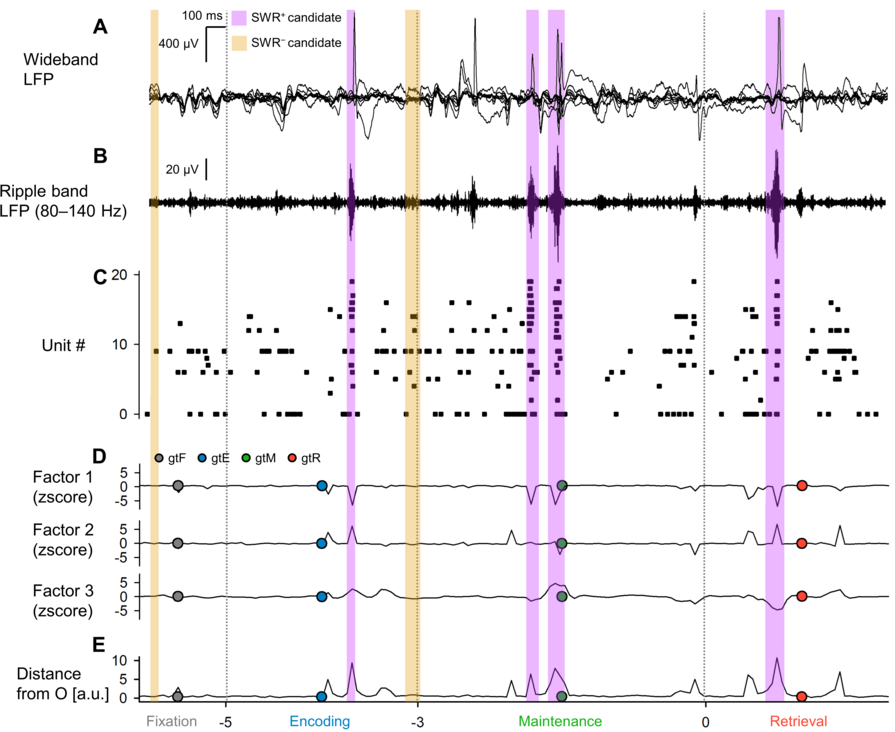
\includegraphics[width=1\textwidth]{./src/figures/.png/Figure_ID_01.png}
        	\caption{\textbf{
Local Field Potentials (LFP), Multiunit Activity, and Neural Trajectories in the Hippocampus During a Modified Sternberg Task
}
\smallskip
\\
\textbf{\textit{A.}} These traces show representative wideband LFP intracranial EEG (iEEG) signals recorded from the left hippocampal head. The subject performed a modified Sternberg working memory task, which includes fixation (1 s, \textit{gray}), encoding (2 s, \textit{blue}), maintenance (3 s, \textit{green}), and retrieval (2 s, \textit{red}). \textbf{\textit{B.}} We then present the corresponding ripple band LFP traces. \textbf{\textit{C.}} The raster plot depicts multiunit spikes taken from the LFP traces, sorted using a spike algorithm \cite{niediek_reliable_2016}. \textbf{\textit{D.}} Subsequently, we illustrate the neural trajectories, which are calculated by GPFA on spike counts per unit with 50-ms bins. Each phase's geometric median is marked by the dot circles. \textbf{\textit{E.}} The trajectory's distance from the origin $O$ is portrayed, with \textit{purple} and \textit{yellow} rectangles indicating the timings for SWR$^+$ candidates and SWR$^-$ candidates (considered as controls for SWR$^+$), respectively.
}
% width=1\textwidth
        	\label{fig:01}
        \end{figure*}
